\documentclass[11pt, a4paper]{article}

\def\ncourse {Numerical Analysis}
\def\ntype {problems}

\makeatletter

% packages
\usepackage{amssymb,amsfonts,amsmath,calc,tikz,pgfplots,geometry,mathtools}
\usepackage{color}   % May be necessary if you want to color links
\usepackage[svgnames]{xcolor}
\usepackage[hidelinks]{hyperref}
\usepackage{forest}
\usepackage{commath} % ew
\usepackage{esvect} % \vv makes vectors
\usepackage{centernot} % for the comparison
\usepackage{esdiff}
\usepackage{esint}
\usepackage{amsthm}
\usepackage{fancyhdr}
\usepackage{bm}
\usepackage{witharrows}
\usepackage{bookmark}
\usepackage{tikz-cd}
\usepackage{quiver}
\usepackage{bbm}
\usepackage{textcomp}
\usepackage{float}
\usepackage{gensymb}
\usepackage{cleveref}
\usepackage{environ}
\usepackage{comment}
\usepackage{cancel}
\usepackage{xparse}

% Inevitable cs
\usepackage{listings}
\usepackage[]{algorithm2e}

% tikz libraries
\usetikzlibrary{positioning}
\usetikzlibrary{matrix}
\usetikzlibrary{arrows}
\usetikzlibrary{bending}
\usetikzlibrary{arrows.meta}
\usetikzlibrary{decorations.markings}
\usetikzlibrary{decorations.pathreplacing}
\usetikzlibrary{decorations.markings}
\usetikzlibrary{patterns}
\usetikzlibrary{backgrounds}

% Page style setup
\pagestyle{fancy}
\fancyhfoffset{0pt}
\renewcommand{\headwidth}{\textwidth}
\geometry{margin=1in}
\pgfplotsset{compat=1.18}
\setlength{\headheight}{14.6pt}
\addtolength{\topmargin}{-1.6pt}
\hypersetup{
    colorlinks=false,
    linktoc=section,
    linkcolor=black,
}

%% maketitle setup
\ifx \nauthor\undefined
  \def\nauthor{Yeheli Fomberg}
\else
\fi

\ifx \nemail\undefined
  \def\nemail{\href{mailto:yp@campus.technion.ac.il}
  {\texttt{<yp@campus.technion.ac.il>}}}
\else
\fi

\ifx \ncoursehead \undefined
  \def\ncoursehead{\ncourse}
\fi

\lhead{\emph{\nouppercase{\leftmark}}}
\ifx \nextra \undefined
  \rhead{
    \ifnum\thepage=1
    \else
      \ncoursehead
    \fi}
\else
  \rhead{
    \ifnum\thepage=1
    \else
      \ncoursehead \ (\nextra)
    \fi}
\fi

\def\notes{notes}
\def\problems{problems}

\ifx \ntype \undefined
  \def\ntype{notes}
\else
\fi

\ifx \ntype \notes
  \let\@real@maketitle\maketitle
  \renewcommand{\maketitle}{\@real@maketitle\begin{center}
  \begin{minipage}[c]{0.9\textwidth}\centering\footnotesize
  These notes are not endorsed by the lecturers.
  I have revised them outside lectures to incorporate supplementary
  explanations, clarifications, and material for fun.
  While I have strived for accuracy, any errors or misinterpretations 
  are most likely mine.
  \end{minipage}\end{center}}
\else
  \ifx \ntype \problems
    \let\@real@maketitle\maketitle
    \renewcommand{\maketitle}{\@real@maketitle\begin{center}
    \begin{minipage}[c]{0.9\textwidth}\centering\footnotesize
    These problems are mostly based on the problem sets I was given
    when taking the course.
    
    While I have strived for accuracy and completeness,
    some of the problems would not have been here without the help of
    friends.
    \end{minipage}\end{center}}
  \else
  \fi
\fi


% theorem environments
\theoremstyle{definition}
\newtheorem{definition}{Definition}[section]
\newtheorem{remark}{Remark}[section]
\newtheorem{example}{Example}[section]
\newtheorem{exercise}{Exercise}[section]
\newtheorem{paradox}{Paradox}[section]
\newtheorem{entry}{Entry}[section]
\newtheorem*{solution}{Solution}
\newtheorem*{question}{Question}
\newtheorem*{answer}{Answer}
\newtheorem*{problem}{Problem}
\theoremstyle{plain}
\newtheorem{theorem}{Theorem}[section]
\newtheorem{proposition}[theorem]{Proposition}
\newtheorem{lemma}[theorem]{Lemma}
\newtheorem{corollary}[theorem]{Corollary}
\newenvironment{proofof}[1]{%
    \renewcommand{\proofname}{Proof of #1}%
    \begin{proof}
}{%
    \end{proof}
}
% tikz customization
\pgfarrowsdeclarecombine{twolatex'}{twolatex'}{latex'}{latex'}{latex'}{latex'}
\tikzset{->/.style = {decoration={markings,
                                  mark=at position 0.999
                                  with {\arrow[scale=2]{latex'}}},
                      postaction={decorate}}}
\tikzset{<-/.style = {decoration={markings,
                                  mark=at position 0.001 with {\arrowreversed[scale=2]{latex'}}},
                      postaction={decorate}}}
\tikzset{-->/.style = {decoration={markings,
                                  mark=at position 0.999
                                  with {\arrow[scale=2]{latex'[sep=0pt -2.5]}}},
                      postaction={decorate}}}
\tikzset{<--/.style = {decoration={markings,
                                  mark=at position 0.001
                                  with {\arrowreversed[scale=2]{latex'[sep=0pt -2.5]}}},
                      postaction={decorate}}}
\tikzset{<->/.style = {decoration={markings,
                                  mark=at position 0.001 with {\arrowreversed[scale=2]{latex'}},
                                  mark=at position 0.999 with {\arrow[scale=2]{latex'}},},
                      postaction={decorate}}}
\tikzset{->-/.style = {decoration={markings,
    mark=at position 0.50+0.225/#1 with {\arrow[scale=2]{latex'}}},
                      postaction={decorate}}}
\tikzset{-<-/.style = {decoration={markings,
                                   mark=at position 0.50-0.225/#1 with {\arrowreversed[scale=2]{latex'}}},
                       postaction={decorate}}}
\tikzset{->>/.style = {decoration={markings,
                                  mark=at position 1 with {\arrow[scale=2]{latex'}}},
                      postaction={decorate}}}
\tikzset{<<-/.style = {decoration={markings,
                                  mark=at position 0 with {\arrowreversed[scale=2]{twolatex'}}},
                      postaction={decorate}}}
\tikzset{<<->>/.style = {decoration={markings,
                                   mark=at position 0 with {\arrowreversed[scale=2]{twolatex'}},
                                   mark=at position 1 with {\arrow[scale=2]{twolatex'}}},
                       postaction={decorate}}}
\tikzset{->>-/.style = {decoration={markings,
                                   mark=at position 0.50+0.450/#1 with {\arrow[scale=2]{twolatex'}}},
                       postaction={decorate}}}
\tikzset{-<<-/.style = {decoration={markings,
                                   mark=at position 0.50-0.450/#1 with {\arrowreversed[scale=2]{twolatex'}}},
                       postaction={decorate}}}

\pgfarrowsdeclare{biggertip}{biggertip}{%
  \setlength{\arrowsize}{1pt}
  \addtolength{\arrowsize}{.1\pgflinewidth}
  \pgfarrowsrightextend{0}
  \pgfarrowsleftextend{-5\arrowsize}
}{%
  \setlength{\arrowsize}{1pt}
  \addtolength{\arrowsize}{.1\pgflinewidth}
  \pgfpathmoveto{\pgfpoint{-5\arrowsize}{4\arrowsize}}
  \pgfpathlineto{\pgfpointorigin}
  \pgfpathlineto{\pgfpoint{-5\arrowsize}{-4\arrowsize}}
  \pgfusepathqstroke
}
\tikzset{
	EdgeStyle/.style = {>=biggertip}
}

\tikzset{circ/.style = {fill, circle, inner sep = 0, minimum size = 3}}
\tikzset{scirc/.style = {fill, circle, inner sep = 0, minimum size = 1.5}}
\tikzset{mstate/.style={circle, draw, black, text=black, minimum width=0.7cm}}

\tikzset{eqpic/.style={baseline={([yshift=-.5ex]current bounding box.center)}}}

\definecolor{mblue}{rgb}{0.2, 0.3, 0.8}
\definecolor{morange}{rgb}{1, 0.5, 0}
\definecolor{mgreen}{rgb}{0, 0.4, 0.2}
\definecolor{mred}{rgb}{0.5, 0, 0}

% topology
\DeclareMathOperator{\dfr}{dfr} % deformation retract
\newcommand{\Cells}{\text{Cells}}
\newcommand{\RP}{\mathbb{RP}}
\newcommand{\CP}{\mathbb{CP}}

% order theory
\newcommand{\join}{\vee}
\newcommand{\meet}{\wedge}

% algebraic geometry
\DeclareMathOperator{\Rad}{Rad} % Radical of modules
\DeclareMathOperator{\Spec}{Spec}
% \renewcommand{\div}{\mathrm{div}} % divisors
\DeclareMathOperator{\Mer}{Mer} % Meromorphic functions
\DeclareMathOperator{\Exc}{Exc} % Exceptional divisor
\DeclareMathOperator{\Td}{Td} % Todd classes

% algebra

\DeclareMathOperator{\trdeg}{tr.deg.}
\DeclareMathOperator{\odd}{odd}
\DeclareMathOperator{\even}{even}
\DeclareMathOperator{\lcm}{lcm}
\DeclareMathOperator{\ord}{ord}
\DeclareMathOperator{\codim}{codim}
\DeclareMathOperator{\Ann}{Ann}
\DeclareMathOperator{\Ext}{Ext}
\DeclareMathOperator{\Sym}{Sym}
\DeclareMathOperator{\Out}{Out}
\DeclareMathOperator{\Aut}{Aut}
\DeclareMathOperator{\End}{End}
\DeclareMathOperator{\Inn}{Inn}
\DeclareMathOperator{\Mat}{Mat}
\DeclareMathOperator{\Fix}{Fix}
\DeclareMathOperator{\std}{std}
\DeclareMathOperator{\sgn}{sgn}
\DeclareMathOperator{\adj}{adj}
\DeclareMathOperator{\id}{id}
\DeclareMathOperator{\op}{op}
\DeclareMathOperator{\tr}{tr}
\DeclareMathOperator{\diag}{diag}
\DeclareMathOperator{\rank}{rank}
\DeclareMathOperator{\rk}{rk}
\DeclareMathOperator{\coker}{coker}
\DeclareMathOperator{\Mult}{Mult} % multiplier algebra
\DeclareMathOperator{\Frac}{Frac} % fraction field
\DeclareMathOperator{\Rat}{Rat}
\DeclareMathOperator{\Gal}{Gal}
\newcommand{\ioplus}{\overset{\text{int}}{\oplus}} % interior direct sum
\newcommand{\GG}{\mathcal G} % Galois correspondence
\newcommand{\FF}{\mathcal F} % Galois correspondence
\newcommand{\cupp}{\smile} % cup product
\newcommand{\capp}{\frown} % cap product
\newcommand{\actson}{\curvearrowright}
\newcommand{\bra}{\left\langle}
\newcommand{\ket}{\right\rangle}
\newcommand{\idealin}{\triangleleft\,}
\newcommand{\normalin}{\triangleleft\,}
\newcommand{\ip}[2]{\left\langle #1, #2 \right\rangle}
\newcommand{\bigslant}[2]
{{\raisebox{.2em}{$#1$}\left/\raisebox{-.2em}{$#2$}\right.}}
\newcommand{\properideal}{%
  \mathrel{\ooalign{$\lneq$\cr\raise.22ex\hbox{$\lhd$}\cr}}}

% categories
\newcommand{\cat}[1]{\mathbf{#1}}
\newcommand{\Ch}{\cat{Ch}} % Chain complexes   
\newcommand{\Set}{\cat{Set}}
\newcommand{\Grp}{\cat{Grp}}
\newcommand{\Ab}{\cat{Ab}}
\newcommand{\Ring}{\cat{Ring}}
\newcommand{\CRing}{\cat{CRing}}
\newcommand{\Top}{\cat{Top}}
\newcommand{\Vect}{\cat{Vect}}
\newcommand{\cmod}{\cat{mod}}

%% matrix groups
\newcommand{\GL}{\mathrm{GL}}
\newcommand{\Or}{\mathrm{O}}
\newcommand{\PGL}{\mathrm{PGL}}
\newcommand{\PSL}{\mathrm{PSL}}
\newcommand{\PSO}{\mathrm{PSO}}
\newcommand{\PSU}{\mathrm{PSU}}
\newcommand{\SL}{\mathrm{SL}}
\newcommand{\msl}{\mathrm{sl}}
\newcommand{\SO}{\mathrm{SO}}
\newcommand{\Spin}{\mathrm{Spin}}
\newcommand{\Sp}{\mathrm{Sp}}
\newcommand{\SU}{\mathrm{SU}}
\newcommand{\U}{\mathrm{U}}
\let\char\relax
\newcommand{\char}{\text{char}}

% analysis
\renewcommand{\Re}{\mathrm{Re}}
\renewcommand{\Im}{\mathrm{Im}}
\NewDocumentCommand{\dx}{o}{
  \IfNoValueTF{#1}
    {\dif x}                  % if no optional argument
    {\dif^{#1} \!x}         % if optional argument
}
\NewDocumentCommand{\dy}{o}{
  \IfNoValueTF{#1}
    {\dif y}                  % if no optional argument
    {\dif^{#1} \!y}         % if optional argument
}
\newcommand{\dt}{\dif t}
\newcommand{\du}{\dif u}
\newcommand{\dv}{\dif v}
\newcommand{\dz}{\dif z}
\newcommand{\ds}{\dif s}
\newcommand{\dw}{\dif w}
\newcommand{\dr}{\dif r}
\newcommand{\dm}{\dif m}
\newcommand{\df}{\dif f}
\newcommand{\dV}{\dif V}
\newcommand{\dS}{\dif S}
\newcommand{\dA}{\dif \mathrm{A}}
\newcommand{\dmu}{\dif \mu}
\newcommand{\dnu}{\dif \nu}
\newcommand{\dtheta}{\dif \theta}
\newcommand{\domega}{\dif \omega}
\newcommand{\dsigma}{\dif \sigma}
\newcommand{\dtau}{\dif \tau}
\newcommand{\dvarphi}{\dif \varphi}
\renewcommand{\dif}{\mathrm{d}}
\renewcommand{\Dif}{\mathrm{D}}
\renewcommand{\triangle}{\Delta}
\newcommand{\ptriangle}{\partial \triangle}
\DeclareMathOperator{\im}{im}
\DeclareMathOperator{\cis}{cis}
\DeclareMathOperator{\rot}{rot}
\DeclareMathOperator{\vspan}{span}
\DeclareMathOperator{\grad}{grad}
\DeclareMathOperator{\curl}{curl}
\DeclareMathOperator{\esssup}{esssup}
\newcommand{\hodge}{{\mathnormal{\star}}}
\DeclareMathOperator{\range}{range}
\DeclareMathOperator{\Hom}{Hom}
\DeclareMathOperator{\Int}{Int}
\DeclareMathOperator{\Conv}{Conv} % convex hull
\newcommand{\ind}{\mathbbm{1}}
\DeclareMathOperator{\Res}{Res}
\DeclareMathOperator{\graph}{graph}
\DeclareMathOperator{\diam}{diam}
\DeclareMathOperator{\supp}{supp}
\DeclareMathOperator{\Vol}{Vol} % Volume
\DeclareMathOperator{\Area}{Area} % Area
\DeclareMathOperator{\area}{area}
\DeclareMathOperator{\Ind}{Ind} % Index
\newcommand{\length}{\mathrm{length}}

% logic
\DeclareMathOperator{\MOD}{MOD}
\DeclareMathOperator{\Theory}{Theory}
\newcommand{\notimplies}{%
  \mathrel{{\ooalign{\hidewidth$\not\phantom{=}$\hidewidth\cr$\implies$}}}}

% nice
\newcommand{\half}{\frac{1}{2}}
\newcommand{\pair}{\del}
\newcommand{\taking}[1]{\xrightarrow{#1}}
\newcommand{\otaking}[1]{\xleftarrow{#1}}
\newcommand{\inv}{^{-1}}
\newcommand{\ot}{\leftarrow}
\newcommand{\ninfty}{-\infty}
\newcommand{\pinfty}{+\infty}
\newcommand{\floor}[1]{\left\lfloor #1 \right\rfloor}
\newcommand{\ceil}[1]{\left\lceil #1 \right\rceil}
\newcommand{\viff}{\Big\Updownarrow} % vertical iff
\newcommand{\bmid}{\,\middle\vert\,} % big mid

% probability
\newcommand{\Prob}{\mathbf{P}}
\renewcommand{\vec}[1]{\boldsymbol{\mathbf{#1}}}
\DeclareMathOperator{\Bin}{Bin}
\DeclareMathOperator{\Geo}{Geo}
\DeclareMathOperator{\Poi}{Poi}
\DeclareMathOperator{\Exp}{Exp}
\DeclareMathOperator{\Var}{Var} % Variance
\DeclareMathOperator{\Cov}{Cov}

% special letters
\newcommand{\N}{\mathbb{N}}
\newcommand{\Z}{\mathbb{Z}}
\newcommand{\Q}{\mathbb{Q}}
\newcommand{\R}{\mathbb{R}}
\newcommand{\C}{\mathbb{C}}
\newcommand{\F}{\mathbb{F}}
\newcommand{\E}{\mathbf{E}}
\newcommand{\D}{\mathbb{D}}
\renewcommand{\H}{\mathbb{H}}
\newcommand{\ps}{\mathcal{P}}
\newcommand{\M}{\mathcal{M}}
\renewcommand{\L}{\mathcal{L}}
\renewcommand{\O}{\mathcal{O}}
\renewcommand{\U}{\mathcal{U}}
\newcommand{\Omicron}{O}
\newcommand{\powerset}{\mathcal{P}}

% text
\newcommand{\st}{\text{ s.t. }}
\newcommand{\tand}{\quad \text{and} \quad}
\newcommand{\tor}{\quad \text{or} \quad}
\newcommand{\stand}{\text{ and }}
\newcommand{\stor}{\text{ or }}
\renewcommand{\tt}[1]{\textnormal{\textbf{(#1).}}} %tt=theorem title GET RID OF

% title format
\title{\textbf{\ncourse}}

\ifx \ntype \notes
  \author{Notes taken by \nauthor\, \nemail \\ Based on lectures by \nlecturer}
  \date{\nterm\ \nyear}
\else
  \ifx \ntype \problems
    \author{These problems were solved by \nauthor \\ \nemail}
  \else
  \fi
\fi

\makeatother

\DeclareMathOperator{\fl}{fl}
\DeclareMathOperator{\NaN}{NaN}

\begin{document}
\maketitle
\newpage
\tableofcontents
\newpage

\section{Digital number representation and non-linear equations}

\begin{exercise}
  Given a computer using base $\beta \in \N$ such that $\beta \geq 2$,
  calculate the unit roundoff error in the computer.
  Recall the numbers are represented as
  \[
    \fl(x) = (-1)^{s} q \cdot \beta^{m}
  \]
  where $s \in \set{0,1}, \beta^{-1} \le q < 1, -126 \le m \le 127$ and
  $q$ is represented as $n$ bits in the computer.
\end{exercise}
\begin{solution}
  We have that
  \[
    x =
    (-1)^{s} \cdot
    \underbrace{(0 . q_1 q_2 \cdots)_{\beta}}_{q < 1} \cdot
    \beta^{m},\quad x \neq 0.
  \]
  Without loss of generality assume $x$ is positive.
  We denote
  \[
    x_- =
    (0 . q_1 q_2 \cdots q_n)_{\beta} \cdot
    \beta^{m}
    \stand
    x_+ =
    (0 . q_1 q_2 \cdots q_n + \beta^{-n})_{\beta} \cdot
    \beta^{m}
  \]
  so
  \[
    |x_- - x_+| = \beta^{m - n}
  \]
  and we have that
  \[
    \fl(x) =
    \begin{cases}
      x_-, &|x - x_-| \le |x - x_+| \\
      x_+, &|x - x_-| > |x - x_+|
    \end{cases}.
  \]
  so without loss of generality we can assume $x$ is closer to $x_-$
  (the calculations in the other case are similar) and we can see that
  \[
    \abs{x - \fl(x)} =
    \abs{x - x_-} \le
    \half |x_- - x_+| =
    \half \beta^{m - n}.
  \]
  Therefore the unit roundoff error is
  \[
    \abs{\frac{\fl(x) - x}{x}} =
    \abs{\frac{x_- - x}{x}} \le
    \frac{\half \beta^{m - n}}{q \beta^{m}} \le
    \frac{\half \beta^{m - n}}{\beta^{-1} \beta^{m}} =
    \half \cdot \beta^{1 - n}.
  \]
  which completes the proof.
\end{solution}

\begin{exercise}
  Find the values of
  \[
    \abs{\frac{\fl(x) - x}{x}} \stand \abs{\fl(x) - x} \stand \fl(x)
  \]
  for $x = 7 / 16$ and $x = 4 / 9$.
\end{exercise}
\begin{solution}
  First we notice that
  \[
    \frac{7}{16} = \frac{1}{16} + \frac{1}{8} + \frac{1}{4}.
  \]
  This means that $x = 7 / 16$ is a machine number.
  Therefore
  \[
    \abs{\frac{\fl(x) - x}{x}} = 0 \stand
    \abs{\fl(x) - x} = 0
    \stand \fl(x) = x = \frac{7}{16}.
  \]
  For $x = 4 / 9$ we see that
  $x = (0.b_1 b_2 \cdots)_{2}$
  and that
  \[ 
    \begin{aligned}
      2 \times \frac{4}{9} &= \frac{8}{9} \quad &&\implies b_1 = 0 \\
      2 \times \frac{8}{9} &= 1 + \frac{7}{9} \quad &&\implies b_2 = 1 \\
      2 \times \frac{7}{9} &= 1 + \frac{5}{9} \quad &&\implies b_3 = 1 \\
      2 \times \frac{5}{9} &= 1 + \frac{1}{9} \quad &&\implies b_4 = 1 \\
      2 \times \frac{1}{9} &= \frac{2}{9} \quad &&\implies b_5 = 0 \\
      2 \times \frac{2}{9} &= \frac{4}{9} \quad &&\implies b_6 = 0 \\
    \end{aligned}
  \]
  Since we reached $4 / 9$ again this process is infinitely repeating and
  thus
  \[
    x = (0.\overline{011100})_{2} \implies
    x = 2^{-2} \cdot (1.\overline{110001})_{2}.
  \]
  Since we have that
  \begin{align*}
    x_- &= (1.11000111000111000111000)_{2} \cdot 2^{-2} \\
    x_+ &= (1.11000111000111000111001)_{2} \cdot 2^{-2}
  \end{align*}
  we get that
  \[
    \abs{x - x_-} =
    2^{-2} \cdot (0.00000000000000000000000\overline{111000}) =
    2^{-24} \cdot (0.0\overline{111000})_2 =
    2^{-24} \cdot \frac{4}{9}.
  \]
  We also have that
  \[
    (x_+ - x) =
    (x_+ - x_-) - (x - x_-)
    \implies
    (x_+ - x) =
    2^{-2} \cdot 2^{-23} - 2^{24} \cdot \frac{4}{9} =
    2^{-25} \cdot \frac{1}{9}.
  \]
  This implies that
  \[
    \fl(x) = x_+ =
    (1.11000111000111000111001)_{2} \cdot 2^{-2}
  \]
  and
  \[
    \abs{\fl(x) - x} =
    x_+ - x =
    \frac{1}{9} \cdot 2^{-25}
  \]
  and finally
  \[
    \abs{\frac{\fl(x) - x}{x}} =
    \frac{\frac{1}{9} \cdot 2^{-25}}{\frac{4}{9}} =
    2^{-27}.
  \]
\end{solution}

\begin{exercise} \phantom{}
\begin{enumerate}
  \item[(1)] Show that the number $0.5$ has two different binary representations
  \item[(2)] Show that a number $x \neq 0$ has a unique binary representation
    if and only if it doesn't have a finite binary representation.
  \item[(3)] How many numbers $x$ are there in the computer execpt the
    special numbers $\pm 0, \pm \infty$.
\end{enumerate}
\end{exercise}
\begin{solution} \phantom{}
\begin{enumerate}
  \item[(1)] We have that
    \[
      (0.1 \overline{00})_{2} = 2^{-1} = \frac{1}{2}
    \]
    and we also have that
    \[
      (0.0\overline{11}) =
      \sum_{i=2}^{\infty} 2^{-i} =
      2^{-1} \cdot \sum_{i=1}^{\infty} 2^{-i} =
      2^{-1} \cdot 1 =
      \frac{1}{2}
    \]
    which shows that $0.5$ has two different binary representations.
  \item[(2)] First suppose that $x$ has a finite binary representation.
    Denote
    \[
      x = (b_1b_2\cdots b_n)_2.
    \]
    Since $x \neq 0$ it is clear from conventions that $b_n = 1$ and then
    we have
    \[
      x =
      (b_1b_2\cdots b_{n-1}1)_2 - 2^{-n} + 2^{-n} =
      (b_1b_2\cdots b_{n-1}1)_2 - 2^{-n} + \sum_{i=1}^{\infty} 2^{-n-i} \\ =
      (b_1b_2 \cdots b_{n-1} 0 \overline{11})_2
    \]
    which shows that $x$ does not have a unique binary representation.

    Next suppose that $x$ does not have a finite binary representation.
    Assume by contradiction that there exist
    \[
      x = (b_1b_2 \cdots)_2 = (c_1c_2 \dots)_2
    \]
    two different infinite binary representations of $x$.
    Then there exists a minimal index $n \geq 1$ such that $b_n \neq c_n$.
    Without loss of generality we have $b_n = 0$ and $c_n = 1$.
    We now see that
    \begin{align*}
      (c_1c_2 \cdots)_2 = (b_1b_2 \cdots)_2 &\implies
      (c_1c_2\cdots c_{n-1} 1 c_{n+1} \cdots)_2 = 
      (c_1c_2\cdots c_{n-1} 0 b_{n+1} \cdots)_2 \\ &\implies
      2^{-n} + 2^{-n} \cdot (c_{n+1} c_{n+2} \cdots)_2 =
      2^{-n} \cdot (b_{n+1} b_{n+2} \cdots)_2.
    \end{align*}
    But since we know that
    \[
      (b_{n+1} b_{n+2} \cdots)_2 \le 2^{-n}
    \]
    it follows that $(c_{n+1} c_{n+2} \dots)_2 = (00\cdots)_2$ which means
    that
    \[
      x = (c_1 c_2 \cdots)_2 = (c_1 c_2 \cdots c_n)_2
    \]
    so there exists a finite binary representation for $x$ which is a
    contradiction.
    Therefore, our assumption is false, which completes the proof.
  \item[(3)] When representing normalized numbers using single precision
    floating points they are represented as such
    \[
      x = (-1)^{s} \cdot q \cdot 2^{m},
    \]
    where $q = (1.f)_2$ and $m = e - 127$.
    We know that there are two possible values for $s$,
    and $2^8 - 2$ possible values for $e$,
    because we want to exclude $\NaN$ and special numbers like
    $\pm 0$ and $\pm \infty$.
    We know that $f$ can have $2^{23}$ possible values and since each
    combination of $s$, $e$ and $m$ represents a different machine number,
    the total amount of different normalized numbers we can represent is
    $2 \times (2^8 - 2) \times 2^{23}$.
    However, when counting denormalized numbers
    (exponent $0$ and the leading bit is not implied),
    there are $2^{23} - 1$ possible values for the mantissa (we exclude $\pm 0$)
    and two for possible values for $s$
    so we can represent $2 \times (2^{23} - 1)$ different denormalized numbers.
    In total we get that the total amount of numbers we can represent is
    \[
      2 \times (254 \times 2^{23} + 2^{23} - 1) =
      4,\!278,\!190,\!078.
    \]
\end{enumerate}
\end{solution}

\begin{exercise}
  Suggest a method to calculate the function $f \colon \R^n \to \R$ defined as
  \[
    f(x_1,x_2,\dots,x_n) = \log\del{\sum_{i=1}^{n} e^{x_i}}
  \]
  such that for any input $x$ it would be possible to calculate $f(x)$
  without calculating positive exponents.
\end{exercise}
\begin{solution}
  Denote
  \[
    1_n :=
    \begin{pmatrix}
      1 & 1 & \cdots & 1
    \end{pmatrix}
  \]
  the $1 \times n$ matrix with $1$ in every entry.
  Let $M \in \R$.
  We have
  \[
    f(x - M \cdot 1_n) =
    \log\del{\sum_{i=1}^{n} e^{x_i- M}} =
    \log\del{e^{-M} \cdot \sum_{i=1}^{n} e^{x_i}}
  \]
  and from properties of logarithms
  \[
    \log\del{e^{-M} \cdot \sum_{i=1}^{n} e^{x_i}} =
    \log\del{e^{-M}} + \log\del{\sum_{i=1}^{n} e^{x_i}} =
    f(x) - M.
  \]
  We now have that
  \[
    f(x) = f(x - M \cdot 1_n) + M.
  \]
  We can now set
  \[
    M = \max_{i \in \set{1,\dots,n}} x_i
  \]
  and then all the exponents we need to calculate to find the value of the
  function will be negative, which reduces the risk of overflows, but
  increases the risk of underflow.
\end{solution}

\begin{exercise}
  Given a polynomial $p(z) = - 3 z^5 + 7 z^4 - 5 z^3 + z^2 - 8 z + 2$,
  \begin{enumerate}
    \item[(1)] Find the values of $p(5)$ and $p'(5)$ using Horner's method.
    \item[(2)] Find the Taylor expansion of $p(z)$ around $z = 3$ using
      Horner's algorithm.
  \end{enumerate}
\end{exercise}
\begin{solution} \phantom{}
\begin{enumerate}
  \item[(1)] We know that we can write
    \[
      p(z) = (z - 5) q(z) + r
    \]
  where $r = b_{-1}$.
  We can see that
  \begin{align*}
    b_4 &= -3 \\
    b_3 &= 7 + 5 \times -3 = -8 \\
    b_2 &= -5 + 5 \times -8 = -45 \\
    b_1 &= 1 + 5 \times -45 = -224 \\
    b_0 &= -8 + 5 \times -224 = -1128 \\
    p(5) = b_{-1} &= 2 + 5 \times -1128 = -5638 
  \end{align*}
  this also gives us that
  \[
    p(z) = (z - 5)(-3 z^4 -8 z^3 - 45 z^2 - 224z - 1128) - 5638.
  \]
  We now have that $p'(5) = q(z)$.
  We can use Horner's method again and see that
  \begin{align*}
    b_3 &= -3 \\
    b_2 &= -8 + 5 \times -3  = -23\\
    b_1 &= -45 + 5 \times -23 = -160 \\
    b_0 &= -224 + 5 \times -160 = -1024 \\
    p'(5) = b_{-1} &= -1128 + 5 \times -1024 = -6248.
  \end{align*}
  \item[(2)] To find the Taylor expansion of $p(z)$ around $z = 3$ we would
    need to find $p(3)$, $p'(3)$, $p''(3)$,\dots,$p^{(5)}(3)$.
    Set $p(z) = (z - 3) q_1(z) + p(3)$.
    According to Horner's method we have
  \begin{align*}
    b_4 &= -3 \\
    b_3 &= 7 + 3 \times -3 = -2 \\
    b_2 &= -5 + 3 \times -2 = -11 \\
    b_1 &= 1 + 3 \times -11 = -32 \\
    b_0 &= -8 + 3 \times -32 = -104\\
    p(3) = b_{-1} &= 2 + 3 \times -104 = -310.
  \end{align*}
  This gives use that $p(3) = -310$ and also that
  \[
    q_1(z) = -3 z^4 - 2 z^3 - 11 z^2 - 32 z - 104.
  \]
  We notice that $p'(3) = q_1(3)$ and then according to Horner's method
  \begin{align*}
    b_3 &= -3 \\
    b_2 &= -2 + 3 \times -3 = -11 \\
    b_1 &= -11 + 3 \times -11 = -44 \\
    b_0 &= -32 + 3 \times -44 = -164\\
    p'(3) = q_1(3) = b_{-1} &= -104 + 3 \times -164 = -596.
  \end{align*}
  This gives use that $p'(3) = q_1(3) = -596$ and also that
  \[
    q_2(z) = -3 z^2 - 11 z^2 - 44 z - 164.
  \]
  for $q_1(z) = (z - 3) q_2(z) + q_1(3)$.
  Recall that we have
  \[
    p(z) = q_1(z) (z - 3) + p(3) \implies
    p'(z) = q_1(z) + q_1'(z) (z - 3).
  \]
  This gives us that
  \[
    p''(z) = q_1'(z) + q_1''(z) (z - 3) + q_1'(z) \implies
    p''(3) = 2 q_1'(3).
  \]
  Similarly we have
  \begin{align*}
    b_2 &= -3 \\
    b_1 &= -11 + 3 \times -3 = -20 \\
    b_0 &= -44 + 3 \times -20 = -104 \\
    q_1'(3) = q_2(3) = b_{-1} &= -164 + 3 \times -104 = -476.
  \end{align*}
  We then have $p''(3) = 2 q_1'(3) = 2 b_{-1} = -952$ and
  \[
    q_3(z) = -3 z^2 - 20 z - 104
  \]
  for $q_2(z) = (z - 3) q_3(z) + q_2(3)$ and we continue in the same way
  \begin{align*}
    b_1 &= -3 \\
    b_0 &= -20 + 3 \times -3 = -29 \\
    q_2'(3) = q_3(3) = b_{-1} &= -104 + 3 \times -29 = -191.
  \end{align*}
  It follows that
  \[
    p'''(3) = 3 q_1''(3) = 3 \cdot 2 \cdot q_2'(3) = 6 \times -191 = -1,\!146
  \]
  and
  \[
    q_4(z) = -3z - 29.
  \]
  And finally
  \begin{align*}
    b_0 &= -3 \\
    q_4(3) = b_{-1} &= -29 + 3 \times -3 = -38.
  \end{align*}
  It follows that
  \[
    p^{(4)}(3) = 4 q_1'''(3) = \cdots = 4! \times q_4(3) = 4! \times -38.
  \]
  We also have
  \[
    q_5(z) = -3 \implies p^{(5)}(3) = 5 ! \times -3.
  \]
  Finally, we have that the Taylor expansion is
  \[
    p(z) = -3 (z - 3)^5 - 38 (z - 3)^4 - 191 (z - 3)^3 - 476 (z - 3)^2
    - 596 (z - 3) - 310.
  \]
\end{enumerate}
\end{solution}

\begin{exercise}
  Write a python program that calculates the values of the functions
  \[
    f(x) = \sqrt{x^2 + 1} - 1 \stand
    g(x) = \frac{x^2}{\sqrt{x^2 + 1} + 1}
  \]
  for $x \in \R$ in single precision.
  Use the function $\texttt{numpy.single()}$ to do calculations in single
  precision.
  \begin{enumerate}
  \item[(1)] Show the graphes of $f(x)$ and $g(x)$ on the same figure for
    $x \in [-1,1]$.
    Calculate the function in $101$ uniformly spreaded points on the interval.
  \item[(2)] Show the graphes of $f(x)$ and $g(x)$ on the same figure for
    $x \in [-0.002,0.002]$.
    Calculate the function in $101$ uniformly spreaded points on the interval.
    Although $f(x)$ and $g(x)$ define the same function the computer gives
    different results.
    Why is that so? Which result is more reliable?
  \item[(3)] Suppose we used double precision instead of single precision
    in our calculations, would the results still be different when the value
    of $x$ is close to $0$?
  \end{enumerate}
\end{exercise}
\begin{solution} \phantom{}
\begin{enumerate}
  \item[(1)] The result is
    \begin{figure}[H]
      \centering
      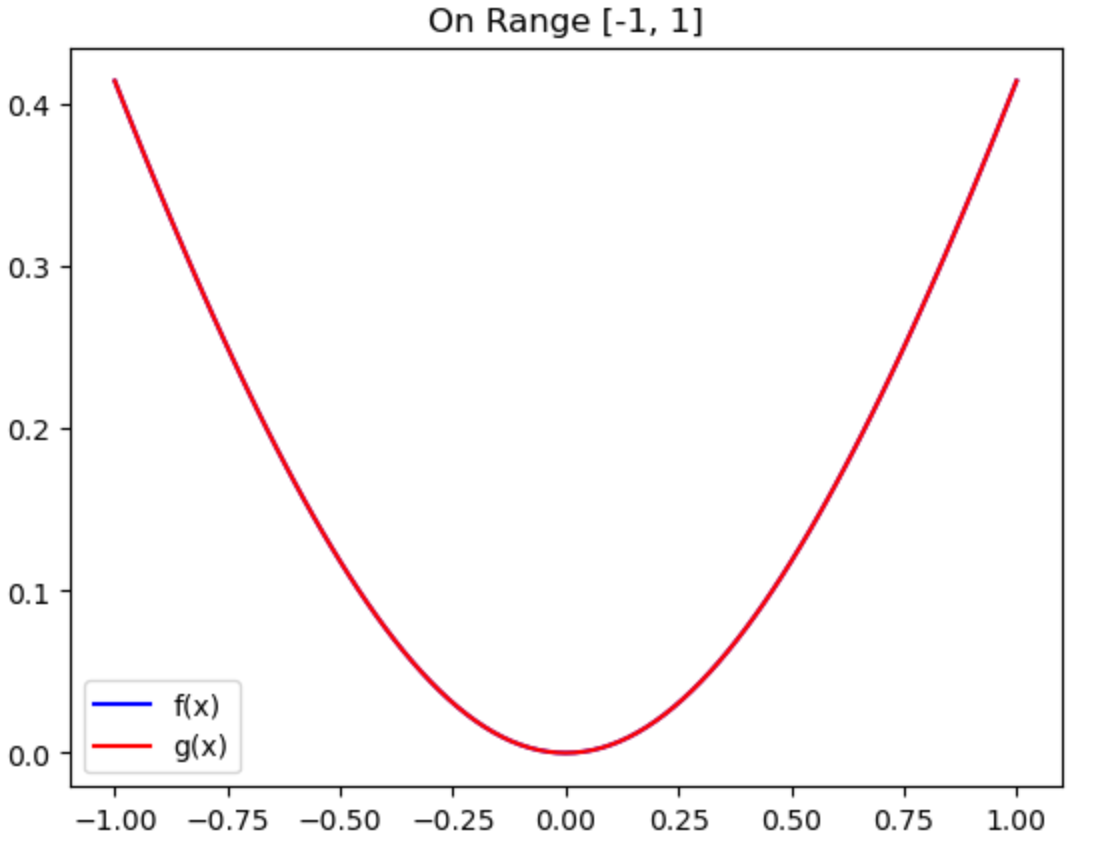
\includegraphics[scale=0.20]{data/widerange}
    \end{figure}
  \item[(2)] The result is now
    \begin{figure}[H]
      \centering
      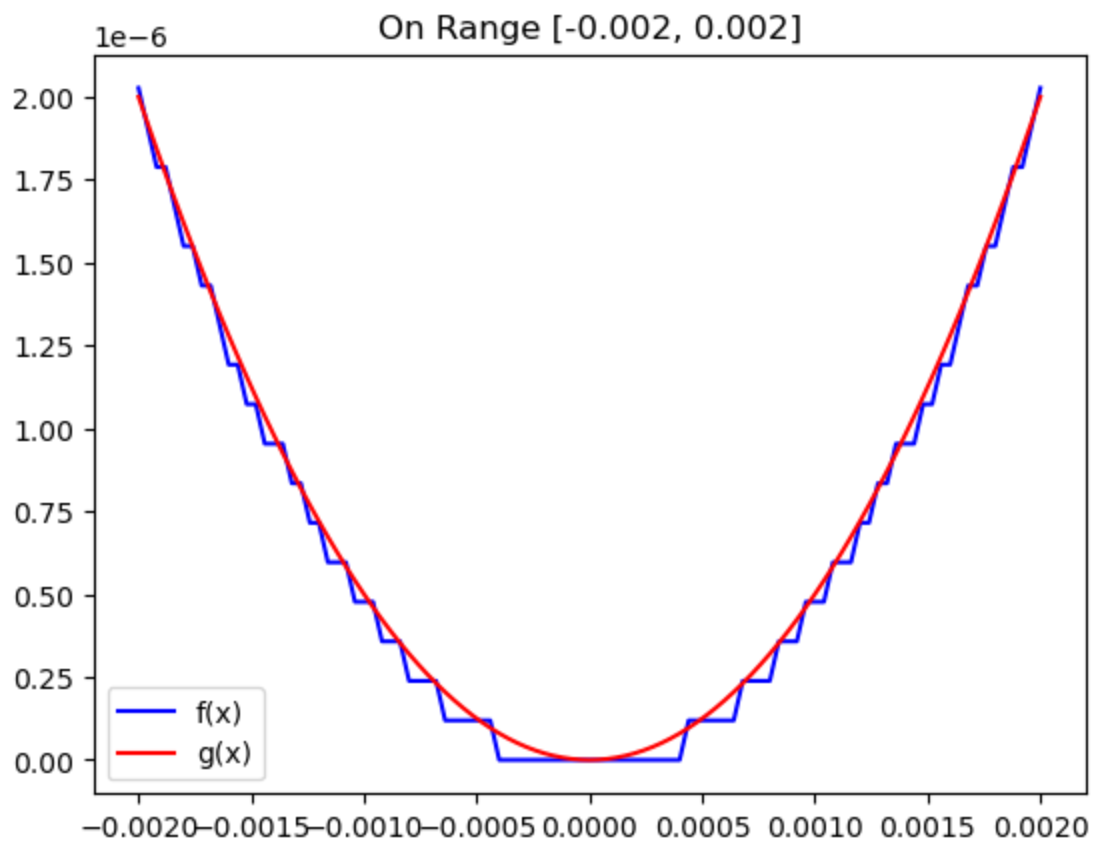
\includegraphics[scale=0.20]{data/narrowrange}
    \end{figure}
    We can see that on the range $[-0.002,0.002]$ the values of the functions
    slightly differ.
    This is because while $f(x)$ uses subtraction---which is a very unstable
    numerical operation when working with floating points---$g(x)$ only
    uses numerically stable operations.
    This makes the values of $g(x)$ more accurate and reliable.
  \item[(3)] If we use double precision the unstability of subtraction would
    not come into a great effect and we would see similar results again.
    However, if we look at smaller values, we would face this problem of
    deviation again.
    We can see this in the following figures:
  \begin{figure}[H]
    \centering
    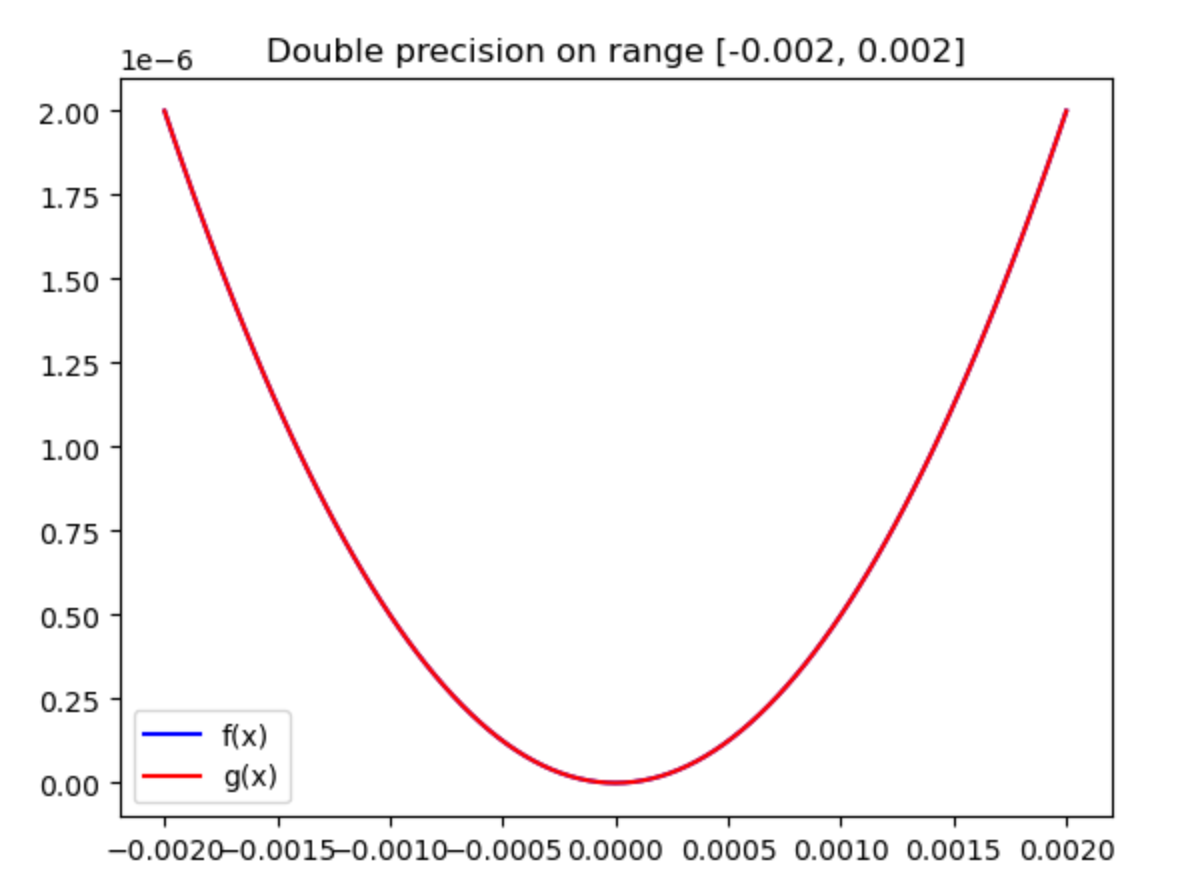
\includegraphics[scale=0.25]{data/doubleprecisionwide}
  \end{figure}
  \begin{figure}[H]
    \centering
    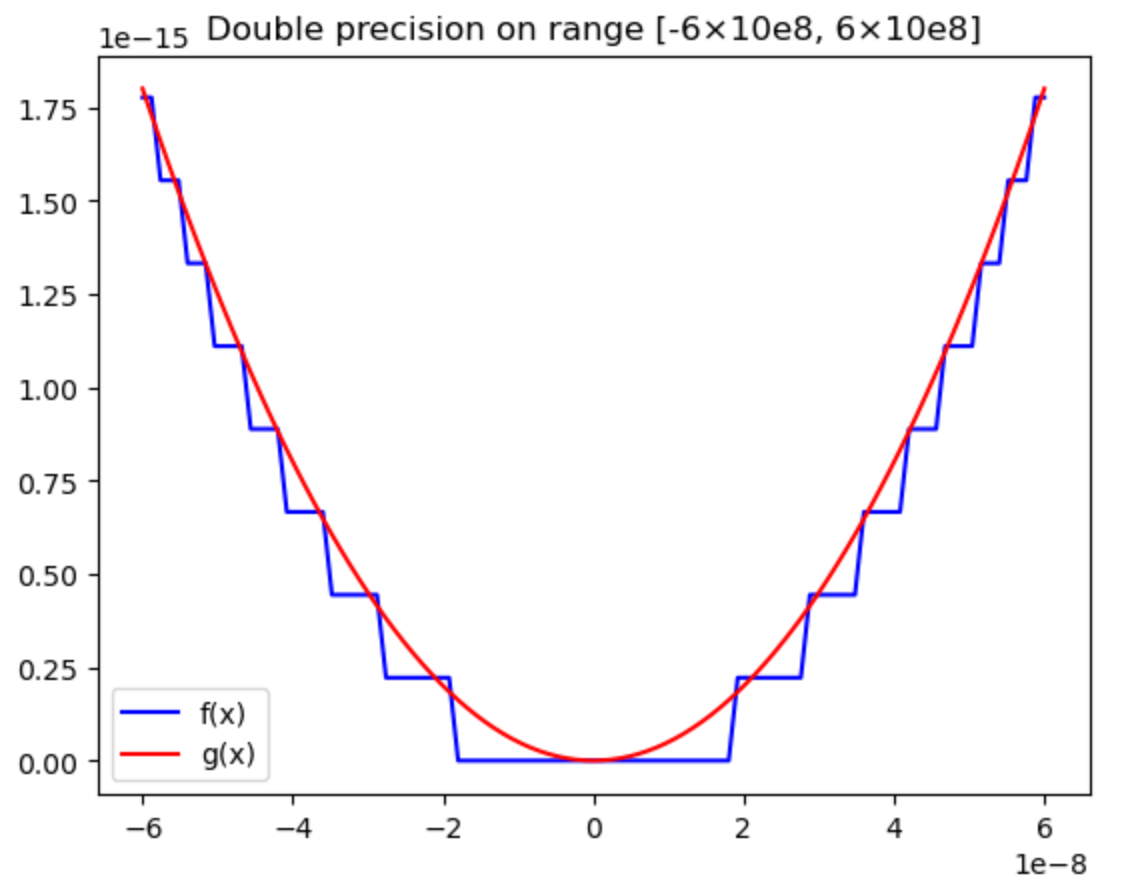
\includegraphics[scale=0.25]{data/doubleprecisionnarrow}
  \end{figure}
\end{enumerate}
\end{solution}

\pgfplotsset{
    myCustomStyle/.style={
        axis lines=middle,
        xlabel={$x$},
        ylabel={$y$},
        samples=100,
        grid=both,
        width=10cm,
        height=6cm,
        enlargelimits=true,
        legend pos=outer north east
    }
}

\newpage
\section{Root-finding algorithms}

\begin{exercise}
  Assuming we apply Newton's method on the following functions
  \begin{enumerate}
    \item[(a)] $f_1(x) = x^5 - x^3 + 3$
    \item[(b)] $f_2(x) = 7x^4 + 3x^2 + \pi$
  \end{enumerate}
  then for each function solve the following problems
  \begin{enumerate}
    \item[(1)] In case we can assume convergence using Newton's
      method, find an interval $I$ such that for all $x \in I$
      we can require convergence.
    \item[(2)] In case there is convergence, what is the convergence rate?
  \end{enumerate}
\end{exercise}
\begin{solution} \phantom{}
\begin{enumerate}
  \item[(b)] We notice that the function in case $(b)$ is smooth
    because it is a polynomial, and we have
    \[
      f_2(x) = 7x^4 + 3x^2 + \pi \geq \pi > 0.
    \]
  Assume by contradiction there exists $x_0$ for which Newton's method
  converge, then
  \[
    \tilde x =
    \lim_{n \to \infty} x_n =
    \lim_{n \to \infty} x_{n+1} =
    \lim_{n \to \infty} \del{x_{n} - \frac{f_2(x_n)}{f_2'(x_n)}} =
    \tilde x - \frac{f_2(\tilde x)}{f_2'(\tilde x)}
  \]
  which means that
  \[
    \tilde x =
    \tilde x - \frac{f(\tilde x)}{f'(\tilde x)}
    \implies
    \frac{f_2(\tilde x)}{f_2'(\tilde x)} = 0
    \implies
    f_2(\tilde x) = 0
  \]
  which is a contradiction to $f_2(x) > 0$ for all $x$.
  This means that an interval of convergence does not exist.

  Since there is no convergence there is also no convergence rate.
  \item[(a)] For case $(a)$ we first find $f_1'(x)$
    \[
      f_1'(x) = 5 x^4 - 3 x^2.
    \]
  Solving for the roots of $f_1'(x)$ we get
  \begin{align*}
             &5 x^4 - 3 x^2 = 0 \\
    \implies &x^2 (5x^2 - 3) = 0 \\ 
      \implies &r_1 = 0 \stand r_{2,3} = \pm \sqrt{\frac{3}{5}}
  \end{align*}
  We approximate (using a computer)
  that one root of $f_1(x)$ is $r \approx -1.42622$ and then
  since we have
  \[
    r < 1 < \min\set{r_1,r_2,r_3} = - \sqrt{\frac{3}{5}}
  \]
  we get that for $\delta_1 = 0.2$ that $f_1'(x)$ doesn't have a root
  on the interval $[r - \delta_1, r + \delta]$.

  Define the function
  \[
    F(x) := x - \frac{f_1(x)}{f_1'(x)}.
  \]
  We now have that
  \begin{align*}
    F'(x) &=
    \frac{\left(20x^{3} - 6x\right)
    \left(x^{5} - x^{3} + 3\right)}{\left(5x^{4} - 3x^{2}\right)^{2}} =
    \frac{2 \left(10x^{2} - 3\right)
    \left(x^{5} - x^{3} + 3\right)}{x^{3} \left(5x^{2} - 3\right)^{2}} \\
    F''(x) &= \frac{2 \left(10x^{7} + 18x^{5} - 750x^{4} + 405x^{2} - 81\right)}
      {x^{4} \left(5x^{2} - 3\right)^{3}}.
  \end{align*}
  This gives that for all $x \in [-3,-1] \ni r$ that $F''(x) < 0$, so
  since $F'(x)$ is continuous and monotonically decreasing on that interval,
  after calculating for $\delta = 0.1$ that
  \[
    F'(r - \delta) = 0.26354 \tand
    F'(r + \delta) = -0.45819
  \]
  it follows that $\abs{F'(x)} < 1$ for any $x$ on the interval
  $[r - \delta, r + \delta]$.
  Thus, since $F(x)$ is a contraction on this interval, Newton's method
  will converge for any $x_0$ we choose on the interval.

  We also have that since the function is in $C^3(\R)$ and the root $r$ is
  simple, by a theorem from class eventually the asymptotic convergence rate
  will be $2$ (quadratic).
\end{enumerate}
\end{solution}

\begin{exercise}
  Does there exist $0 \neq x_0 \in \R$ such that the following interations
  converge? If so, find an interval such that the iterations converge
  for any starting point in the interval, and find the value to which they
  converge.
  \[
    (a)\quad\! x_{n+1} = \frac{1}{3} \del{2 x_n - \frac{r}{x_n^2}},\, r >0 \tand
    (b)\quad\! x_{n+1} = 1 + \frac{2}{x_n}
  \]
\end{exercise}
\begin{solution} \phantom{}
\begin{enumerate}
\item[(a)]
  For sequence $(a)$ we begin by defining
  \[
    F(x) := \frac{1}{3} \del{2 x - \frac{r}{x^2}} \st x_{n+1} = F(x_n).
  \]
  After solving $F(x) = x$ we get that the only solution is
  $R = - \sqrt[3]{r}$.

  We know that if we find some $\delta > 0$ such that the derivative of $F$ is
  strictly smaller than $1$ on the closed interval $[R - \delta, R + \delta]$
  we get that $F$ is a contraction on the interval and thus the sequence
  converges to $R$ for any starting point from that interval.

  First notice that
  \[
    F'(x) = \frac{2}{3} \del{1 + \frac{r}{x^3}}
  \]
  and thus for any $x \in (-\infty, -\sqrt[3]{r / 2}]$ we have that
  \[
    \frac{2}{3} \geq
    F'(x) \geq
    F'\del{- \sqrt[3]{\frac{r}{2}}} =
    \frac{2}{3} (1 - 2) =
    - \frac{2}{3}.
  \]
  This means that for $\delta = -\sqrt[3]{r / 2}$ we have that
  $[R - \delta, R + \delta] \subset (-\infty, -\sqrt[3]{r / 2}]$ and
  that the derivative of $F'$ is strictly smaller than $1$, this means
  that $F$ is a contraction on that interval and then by the Banach fixed-point
  theorem we have that iterations initialized in the interval will converge
  to $R$.
\item[(b)] For sequence $(b)$ we define
  \[
    F(x) := 1 + \frac{2}{x}.
  \]
  We see that it has two fixed points at $x_1 = -1$ and $x_2 = 2$.
  The derivative of $F$ is
  \[
    F'(x) = - \frac{2}{x^2}.
  \]
  We see that $\abs{F'(2)} < 1$ and thus since $F'(x)$ is continuous we
  can find a suitable interval in which the iterations will converge.

  Let $R$ be a number such that $\sqrt 2 < R < 2$.
  Then we have $2 \in I = [R,\infty)$ and for any $x$ in $I$ we have
  \[
    \abs{F'(x)} \le
    \frac{2}{R^2} <
    \frac{2}{\del{\sqrt 2}^2} = 1.
  \]
  We can now reduce $I$ to a symmetrical interval around the
  fixed point by choosing $\delta = 2 - R$ and setting the interval
  $[2 - \delta, 2 + \delta]$.

  In this new interval $F$ is a contractive, so the iterations must converge
  to the single fixed point $2$.
\end{enumerate}
\end{solution}

\begin{exercise}
  Suppose we want to calculate $\lim_{n \to \infty} x_n = x^*$ where
  \begin{align*}
    x_0 &= 4^{1/3} \\
    x_1 &= \del{4^{2/3} + 4}^{1/3} \\
    x_2 &= \del{\del{4^{2/3} + 4}^{2/3} + 4}^{1/3} \\
    x_3 &= \del{\del{\del{4^{2/3} + 4}^{2/3} + 4}^{2/3} + 4}^{1/3} \\
        &\vdotswithin{=}
  \end{align*}
  Define a function $F(x)$ and find an interval $[a,b]$ such that
  $x^* \in [a,b]$ is the limit of $\set{x_n}_{n=0}^{\infty}$ defined by
  $x_{n+1} = F(x_n)$ for $n \geq 0$ for an arbitrary $x_0 \in [a,b]$.
  What is the value of $x^*$.
\end{exercise}
\begin{solution}
  We define the function
  \[
    F(x) := (x^2 + 4)^{1/3}.
  \]
  For $x_0 = 4^{1/3}$ the sequence $x_n$ satisfies $x_{n+1} = F(x_n)$.
  Since $F(x)$ is continuous
  \[
    x^* = \lim_{n \to \infty} x_n
  \]
  The fixed point satisfies $x^* = F(x^*)$ so
  \[
    x^* = \del{(x^*)^2 + 4}^{1/3} \implies
    (x^*)^3 - (x^*)^2 - 4 = 0 \implies
    x^* = 2.
  \]
  Since for all $x \in I := [2 - 0.5, 2 + 0.5]$ we have that $F'(x)$ exists and
  \[
    0 < \frac{1}{3} (x^2 + 4)^{-2/3} \cdot 2x = F'(x)
  \]
  it is also monotonically increasing on $I$.
  Considering that
  \[
    F(1.5) = 1.84201 \tand
    F(2.5) = 2.17224
  \]
  it is clear that $F(I) \subset [F(1.5),F(2.5)] \subset [1.5,2.5]$ so
  $F \colon [1.5,2.5] \to [1.5,2.5]$ is well defined.

  We notice that for $x \in I$
  \begin{align*}
    F'(x) &= \frac{2}{3} x \cdot (x^2 + 4)^{-2/3}
    \le \frac{2}{3} \cdot 2.5 \del{(2.5)^2 + 4}^{-2/3} \\ &=
    \frac{2}{3} \cdot \frac{5}{2} \cdot 0.21192 =
    0.35320 < 1.
  \end{align*}
  Thus, according to Lagrange's theorem, for any $x,y \in I$ there exists
  some $t \in (x,y) \subset I$ such that
  \[
    \abs{F(x) - F(y)} =
    \abs{F'(t)} \cdot \abs{x - y} <
    0.4 \cdot \abs{x - y}
  \]
  the map is contractive with contraction factor $0.4$ on $I$, and since
  we have also already shown that $F \colon I \to I$ is well defined
  ($F(I) \subset I$) we get that $\set{x_n}_{n=0}^{\infty} \subset I$ defined by
  $x_{n+1} = F(x_n)$ for $n \geq 0$ for an arbitrary $x_0 \in I$ that
  $x_n$ converges to $x^* = 2$ which completes the exercise.
\end{solution}

\begin{exercise}
  Given a function $F(x) \in C^1(\R)$ and a fixed point $s$ of $F(x)$,
  prove that if $|F'(s)| \le \lambda < 1$ for $0 < \lambda < 1$ then
  there exists $\epsilon > 0$ such that for all $x_0$ such that
  $|x_0 - s| \le \epsilon$, the functional iterations $x_{n+1} = F(x_n)$
  for $n \geq 0$ converge to $s$.
\end{exercise}
\begin{solution}
  Since $|F'(s)| \le \lambda < 1$ and $F \in C^1(\R)$ we get that there exists
  $\epsilon > 0$ and $0 < c < 1$ such that for all
  $x \in I := [s - \epsilon, s + \epsilon]$ we have
  \[
    \abs{F'(x)} < c < 1.
  \]
  From Lagrange's theorem we have that for all
  $x,y \in I$ that there exists $t \in (x,y)$
  such that
  \[
    F(y) - F(x) = F'(t) (x - y) \implies
    \abs{F(x)- F(y)} = \abs{F'(t)} \cdot \abs{x - y} < c \abs{x - y}
  \]
  for $0 < c < 1$ (because $(x,y) \subset I$).
  This proves that $F$ is a contraction on $I$.

  Let $x \in I = [s - \epsilon, s + \epsilon]$.
  \[
    \abs{F(x) - s} =
    \abs{F(x) - F(s)} \le
    \lambda \abs{x - s} <
    \abs{x - s} <
    \epsilon \implies F(x) \in I.
  \]
  This implies that $F(I) \subseteq I$.

  Finally, we have shown that $F \colon I \to I$ is a contraction mapping,
  and thus according to the contraction mapping theorem every sequence
  $\set{x_n}_{n \in \N} \subset I$ of the form $x_{n+1} = F(x_n)$ converges to
  the fixed point $s$ which completes the exercise.
\end{solution}

\begin{exercise}
  Given a system of equations
  \[
    \begin{cases}
      4 {x_1}^2 - 20 x + \frac{1}{4} {x_2}^2 = -8 \\
      \half x_1 {x_2}^2 + 2 x_1 - 5 x_2 = -8
    \end{cases}
  \]
  Use Newton's method for $x^{(0)} = (0,0)^T$ and calculate $x^{(2)}$.
\end{exercise}
\renewcommand{\arraystretch}{1.25}
\begin{solution}
  Define $F \colon \R^2 \to \R^2$ by
  \[
    F(x) = F(x_1,x_2) =
    \begin{pmatrix}
      4 {x_1}^2 - 20 x + \frac{1}{4} {x_2}^2 + 8 \\
      \half x_1 {x_2}^2 + 2 x_1 - 5 x_2 + 8
    \end{pmatrix}.
  \]
  Calculating the Jacobian we get
  \[
    J_F\del{x} =
    \begin{pmatrix}
      8 x_1 - 20 & \half x_2 \\
      \half x_2^2 + 2 & x_2 x_1 - 5
    \end{pmatrix}.
  \]
  Therefore,
  \[
    F\del{x^{(0)}} =
    \begin{pmatrix}
      8 \\ 8
    \end{pmatrix} \tand
    J_F\del{x^{(0)}} =
    \begin{pmatrix}
      -20 & 0 \\
      2 & -5
    \end{pmatrix}.
  \]
  According to the algorithm we now have
  \[
    x^{(1)} = x^{(0)} + h^{(0)} \quad\text{for}\quad
    J_F\del{x^{(0)}} h^{(0)} = - F\del{x^{(0)}}.
  \]
  Solving the equation we get
  \[
    \begin{pmatrix}
      -20 & 0 \\
      2 & -5
    \end{pmatrix}
    \begin{pmatrix}
      h^{(0)}_1 \\ h^{(0)}_2
    \end{pmatrix} =
    \begin{pmatrix}
      -8 \\ -8
    \end{pmatrix} \implies
    \begin{pmatrix}
      h^{(0)}_1 \\ h^{(0)}_2
    \end{pmatrix} =
    \begin{pmatrix}
      \frac{4}{10} \\ \frac{44}{25}
    \end{pmatrix}
  \]
  so
  \[
    x^{(1)} = x^{(0)} + h^{(0)} =
    \begin{pmatrix}
      0 \\ 0
    \end{pmatrix} +
    \begin{pmatrix}
      \frac{4}{10} \\ \frac{44}{25}
    \end{pmatrix} =
    \begin{pmatrix}
      \frac{4}{10} \\ \frac{44}{25}
    \end{pmatrix}.
  \]
  Similarly we see that
  \[
    F\del{x^{(1)}} =
    \begin{pmatrix}
      \frac{884}{625} \\ \frac{1936}{3125}
    \end{pmatrix} \tand
    J_F\del{x^{(1)}} =
    \begin{pmatrix}
      -\frac{84}{5} & \frac{22}{25} \\
      \frac{2218}{625} & -\frac{537}{125}
    \end{pmatrix}.
  \]
  According to the algorithm we now have
  \[
    x^{(2)} = x^{(1)} + h^{(1)} \quad\text{for}\quad
    J_F\del{x^{(1)}} h^{(1)} = - F\del{x^{(1)}}.
  \]
  Solving the equation we get
  \[
    \begin{pmatrix}
      -\frac{84}{5} & \frac{22}{25} \\
      \frac{2218}{625} & -\frac{537}{125}
    \end{pmatrix}
    \begin{pmatrix}
      h^{(0)}_1 \\ h^{(0)}_2
    \end{pmatrix} =
    \begin{pmatrix}
      -\frac{884}{625} \\ -\frac{1936}{3125}
    \end{pmatrix} \implies
    \begin{pmatrix}
      h^{(0)}_1 \\ h^{(0)}_2
    \end{pmatrix} =
    \begin{pmatrix}
      0.09589 \\ 0.22342
    \end{pmatrix}
  \]
  so
  \[
    x^{(2)} = x^{(1)} + h^{(1)} =
    \begin{pmatrix}
      \frac{4}{10} \\ \frac{44}{25}
    \end{pmatrix} +
    \begin{pmatrix}
      0.09589 \\ 0.22342
    \end{pmatrix} =
    \begin{pmatrix}
      0.49589 \\ 1.98342
    \end{pmatrix}.
  \]
\end{solution}

\begin{exercise} \phantom{}
\begin{enumerate}
  \item[(1)] Find the number of real roots of the function
    \[
      f(x) = -0.2 + x^2 - 4x \sin(x) + \left[2 \sin(x)\right]^2.
    \]
    You may use graphical estimation.
  \item[(2)] Write a python program to find the first positive root of
    $f(x)$ with an error margin of $10^{-6}$.
    Choose starting and termination conditions, as well as $N$, $\epsilon$, 
    $\delta$, and find the root using the bisection method, Newton's method,
    and the Secant method.
    Use $k$ to denote the number of iterations needed to reach the desired
    accuracy, and explain the choice of $N$, $\epsilon$, $\delta$.
\end{enumerate}
\end{exercise}
\begin{solution} \phantom{}
  \begin{enumerate}
  \item[(1)] Using a graphical estimation, we see that the graph of the
    function looks like
    \begin{figure}[H]
    \begin{center}
  \begin{tikzpicture}
    \begin{axis}[myCustomStyle,
        xmin=-3, xmax=3,
        ymin=-1, ymax=1,
        domain=-3:3]
      \addplot[blue, thick] {-0.2 + x^2 - 4*x*sin(deg(x)) + (2*sin(deg(x)))^2};
      \addlegendentry{$f(x)$}
    \end{axis}
  \end{tikzpicture}
    \end{center}
    \end{figure}
    we can see that the function $f(x)$ has $6$ roots.
  \item[(2)] We implemented the root-finding algorithms in python and now
    we need to find the right conditions for them to converge in order for
    this to work. Denote the first positive root of $f(x)$ as $r$.
    We notice that $r \approx 0.5$.
    We also calculate
    \begin{align*}
      f'(x) &= 8 \cos\left(x\right) \sin\left(x\right) -
      4 \sin\left(x\right) - 4x \cos\left(x\right) + 2x.
    \end{align*}

    For the bisection method all we care about is that $a < r < b$
    and that no other roots are in $[a,b]$.
    We notice that
    \begin{center}
  \begin{tikzpicture}
    \begin{axis}[myCustomStyle,
        xmin=0.3, xmax=0.7,
        ymin=-0.1, ymax=0.1,
        domain=0.3:0.7]
      \addplot[blue, thick] {-0.2 + x^2 - 4*x*sin(deg(x)) + (2*sin(deg(x)))^2};
      \addlegendentry{$f(x)$}
    \end{axis}
  \end{tikzpicture}
    \end{center}
    so we can choose $a = 0.4$ and $b = 0.6$ as the starting conditions.
    Since our tolerance is $\epsilon = 10^{-6}$ we get that
    \[
      N \geq \log_2\del{\frac{b - a}{\epsilon}} \approx 17.6096
    \]
    so we can choose $N = 20$.

    For Newton's method we can first see that
    \begin{center}
  \begin{tikzpicture}
    \begin{axis}[myCustomStyle,
        xmin=0.45, xmax=0.50,
        ymin=0.65, ymax=0.70,
        domain=0.45:0.50]
      \addplot[blue, thick] {2*x + 8*sin(deg(x))*cos(deg(x)) - 4*sin(deg(x))
        - 4*x*cos(deg(x))};
      \addlegendentry{$f'(x)$}
    \end{axis}
  \end{tikzpicture}
    \end{center}
    since $f \in C^2(\R)$ and since we see from the graph that it is strictly
    increasing and strictly convex, it follows that Newton's method must
    converge to the root $r$ from any starting point on that interval.
    We will set the initial guess to be $x_0 = 0.475$.
    Since our tolerance is $\epsilon = 10^{-6}$ we will choose $N = 10$
    which is slightly less from the $N$ for the bisection method because
    the convergence rate of Newton's method is quadratic which is faster than
    the linear convergence rate of the bisection method.

    For the secant method we choose two guesses from the same interval as
    in Newton's method because it is close in about $2$ orders of magnitude to
    the root we are looking for.
    We will set $N = 15$ because the convergence rate of the secant method
    is $1 < \varphi \approx 1.618 < 2$ which is subquadratic but superlinear.

    The results of the program are collected here
    \begin{figure}[H]
      \centering
      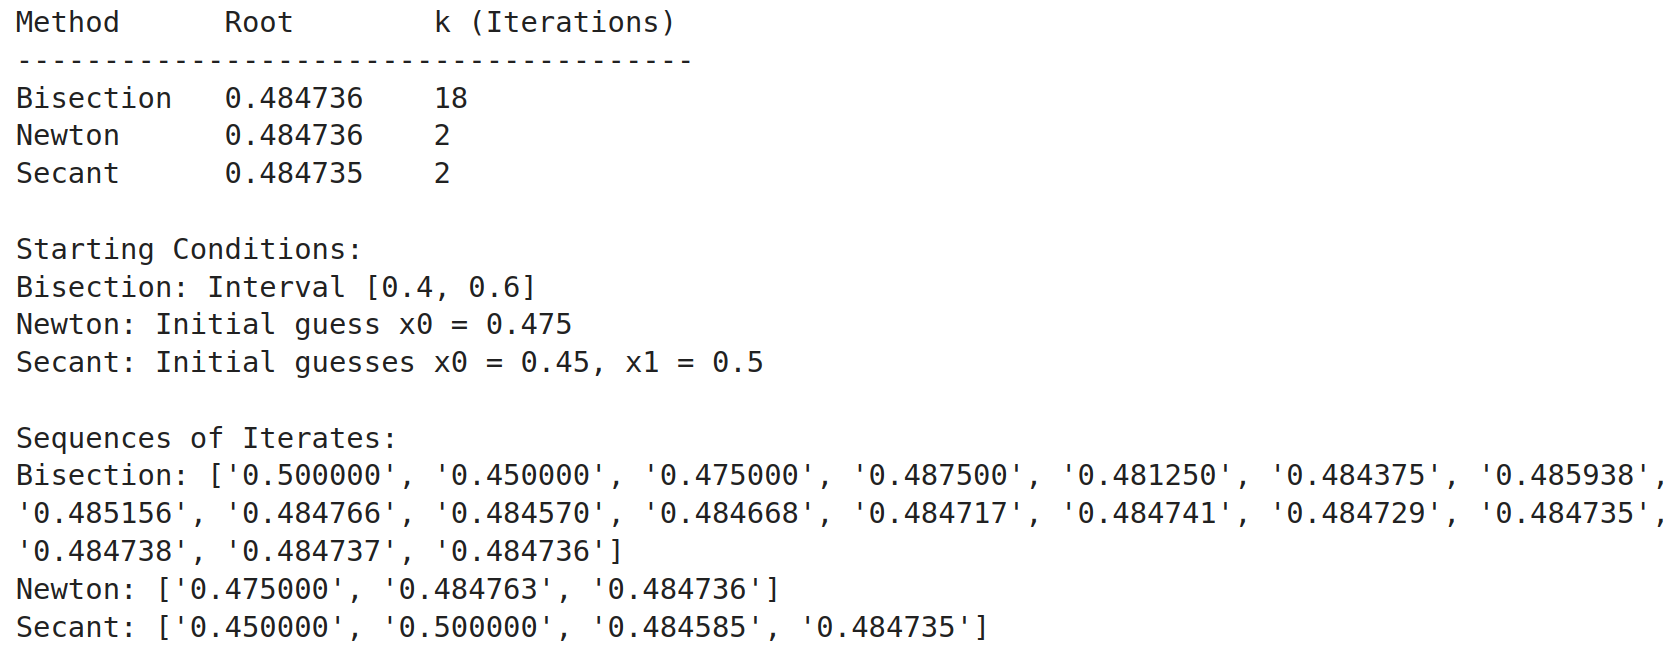
\includegraphics[scale=0.25]{data/hw2data}
    \end{figure}
  \end{enumerate}
\end{solution}


\newpage
\section{Numerical linear algebra}

\begin{exercise}
  Let $f \in C^4(\R)$ and let $r \in \R$ be a root of $f(x)$.
  Find a sufficient condition that $f(x)$ could satisfy at $r$
  so that for $x_0$ close enough to $r$ the applying Newton's method
  on $x_0$ will give a convergence rate of at least $3$.
\end{exercise}
\begin{solution}
  In order to use Newton's method we first require $f'(x) \neq 0$ in
  a neighbourhood of the root.
  Since we want it to converge we also require $\abs{f'(x)} < 1$ around the
  root.
  Consider the function
  \[
    F(x) := x - \frac{f(x)}{f'(x)}.
  \]
  Accodring to Taylor's theorem we have
  \[
    F(x) = F(r) + F'(r)(x - r) + \half F''(r)(x - r)^2 + R_2(x).
  \]
  Writing the remainder in Lagrange's form gives
  \[
    F(x) = F(r) + F'(r)(x - r) + \half F''(r)(x - r)^2 +
    \frac{F^{(3)}(c)}{3!}(x - r)^3
  \]
  for some $c$ between $x$ and $r$.
  After computation and assuming $f''(r) = 0$ we have
  \begin{align*}
    F(r) &= r - \frac{f(r)}{f'(r)} = r \\
    F'(r) &= 1 - \frac{(f'(r))^2 - f(r)f''(r)}{(f'(r))^2} = 1 - 1 = 0 \\
    F''(r) &=
    \frac{(f'(r))^3 f''(r) + (f'(r))^2 f(r) f^{(3)}(r) - 2 f'(r) f(r) 
    (f''(r))^2}{(f'(r))^4} = 0
  \end{align*}
  this gives us
  \[
    F(x) = r + \frac{F^{(3)}(c)}{3!}(x - r)^3.
  \]
  Let $\set{x_n}_{n=0}^{\infty}$ be the sequence resulting from Newton's
  method.
  Since $x_{n+1} = F(x_n)$ we get that
  \[
    \abs{x_{n+1} - r} =
    \abs{F(x_n) - r} =
    \abs{\frac{F^{(3)}(c_n)}{3!}(x_n - r)^3} \le
    \abs{\frac{F^{(3)}(c_n)}{3!}}\abs{x_n - r}^3.
  \]
  Since $f \in C^4(\R)$ the function $f^{(3)}$ is continuous around $r$
  so since from the contractive mapping theorem we have
  $c_n \taking{n \to \infty} r$ we get
  $f^{(3)}(c_n) \taking{n \to \infty} f^{(3)}(r)$.
  It follows that if we require $f^{(3)}(r) \neq 0$ then
  exists $C = \half f^{(3)}(r) > 0$ and $N > 0$ such that for all
  $n > N$ we have
  \[
    \abs{x_{n+1} - r} \le
    C \abs{x_n - r}^3
  \]
  which means we have cubic convergence and completes the proof.
\end{solution}

\begin{exercise}
  Let $p(z) = 2 z^6 + 2 z^5 - 4 z^4 - 12 z^3 + 3 z^3 + 9 z$.
  \begin{enumerate}
    \item[(1)] Find an open annulus in the complex plane that contains all the
      roots of $p(z)$ excluding $0$.
    \item[(2)] Given a polynomial $p(z) \in \C[z]$ of degree $n$ set
      \[
        R := \frac{\abs{a_0} + \abs{a_1} + \cdots + \abs{a_{n-1}}}{\abs{a_n}}.
      \]
      Show that every root $z_0$ of $p(z)$ satisfies
      \[
        \abs{z_0} \le \max\set{R,\sqrt[n]{R}}.
      \]
  \end{enumerate}
\end{exercise}
\begin{solution} \phantom{}
  \item[(1)] According to a theorem from the recitations,
    given a polynomial $p \in \C[z]$ of degree $n$ with coefficients
    $\set{a_i}_{i=0}^{n}$ we can set 
    \[
      \rho := 1 + \frac{1}{|a_n|} \max_{0 \le i < n} |a_i|
    \]
    and then all the roots of $p(z)$ are within $B_{\rho}(0)$.
    Furthermore, if all the roots of $s(z) := z^n p(1/ z)$,
    are within $B_{\bar \rho}(0)$,
    then the roots of $p(z)$ besides $0$ are outside $B_{\bar \rho^{-1}}(0)$.
    We see that for our specific polynomial
    \[
      \rho = 1 + \half \cdot 12 = 7.
    \]
    Since the radius of $s$ is
    \[
      \rho_s = 1 + \frac{1}{9} \cdot 12 = \frac{7}{3}
    \]
    then all roots of $s$ are contained within $B_{\rho_s}(0)$,
    which implies that all roots of $p$ execpt $0$ are contained within the
    annulus
    \[
      A = \set{z \in \C \mid \frac{3}{7} \leq |z| \leq 7}.
    \]
  \item[(2)] 
  Let $z_0$ be a root of $p(z) = \sum_{i=0}^{n} a_i x^i$.
  Since $p(z_0) = 0$ we get that
  \begin{align*}
    a_n z_0^n = - \sum_{i=0}^{n-1} a_i z_0^i &\implies
    |a_n z_0^n| =
    \abs{\sum_{i=0}^{n-1} a_iz_0^i} \leq
    \sum_{i=0}^{n-1} |a_iz_0^i| \\
    &\implies
    |a_n| |z_0|^n =
    |a_n z_0^n| \leq
    \sum_{i=0}^{n-1} |a_i z_0^i|
  \end{align*}
  and so if $|z| < 1$ we have
  \begin{align*}
    |a_n| |z_0|^n =
    |a_n z_0^n| \leq
    \sum_{i=0}^{n-1} |a_i z_0^i| \leq
    \sum_{i=0}^{n-1} |a_i|
    \implies
    |z_0|^n \leq \frac{\sum_{i=0}^{n-1}|a_i|}{|a_n|} = R
    \implies
    |z| \leq \sqrt[n]{R}.
  \end{align*}
  Otherwise, we get that $|z| \geq 1$ so for all $0 \le i \le n - 1$ we have
  \[
    * \quad \frac{|z|^i}{|z|^{n-1}} \leq 1.
  \]
  Using this, we can now obtain that
  \begin{align*}
      |a_n||z_0|^n = |a_nz_0^n|\leq \sum_{i=0}^{n-1}|a_iz_0^i|
      &\implies
      |a_n||z_0| \leq
      \sum_{i=0}^{n-1}|a_i| \frac{|z_0|^i}{|z_0|^{n-1}} \underset{*}{\leq}
      \sum_{i=0}^{n-1}|a_i| \\
      &\implies
      |z_0| \leq \frac{\sum_{i=0}^{n-1}|a_i|}{|a_n|} = R
  \end{align*}
  and so we have $z_0 \leq \max\set{R, \sqrt[n]{R}}$ which completes the
  proof.
\end{solution}

\begin{exercise}
  Let $A,B \in \R^{n \times n}$.
  \begin{enumerate}
    \item[(1)] Show that $\rho(A) \le \norm{A}_2$,
      where $\rho(A) = \max\set{\abs{\lambda_i}}_{i=1}^{n}$ is the spectral
      radius of $A$, and $\set{\lambda_i}_{i=1}^{n}$ are the eigenvalues
      of $A$.
      Moreover, show that if $A$ is symmetric then the equality holds.
    \item[(2)] Show that $A$ is a positive definite and $B$ is non-singular
      if and only if the matrix $B A B^T$ is positive definite.
  \end{enumerate}
\end{exercise}
\begin{solution} \phantom{}
  \item[(1)] Let $V_\lambda$ denote the space of eigenvectors corresponding to
  and eigenvalue $\lambda$.
  \[
    \norm{A}_2 =
    \max_{\norm{x}_2=1} \norm{Ax}_2 \geq
    \max_{\substack{\norm{x}_2=1 \\ x \in V_\lambda}} \norm{Ax}_2 =
    \max_{\substack{\norm{x}_2=1 \\ x \in V_\lambda}} \norm{\lambda x}_2 = \lambda
  \]
  this holds for any $\lambda$ eigenvalue of $A$,
  which in particular implies that
  \[
    \norm{A}_2 \geq \rho(A) = \max\set{\abs{\lambda_i}}_{i=1}^{n}.
  \]
  Let $\set{\sigma_i}_{i=1}^{n}$ denote the singular values of $A$.
  We know that
  \[
    \norm{A}_{2} = \sigma_{\max} = \sqrt{\max \lambda_i(A A^T)}.
  \]
  But since $A$ is symmetric we get that $A A^T = A^2$, which means
  \[
    \norm{A}_{2} =
    \sqrt{\max \lambda_i(A A^T)} =
    \sqrt{\max \lambda_i(A^2)} =
    \max\set{\abs{\lambda_i}}_{i=1}^{n} =
    \rho(A).
  \]
  where the second to last equality holds because
  the eigenvalues of $A^2$ are the eigenvalues of $A$ squared
  and since the number of eigenvalues is finite,
  the max of the square of the values is the square of their max.
  \item[(2)] First suppose that $A$ is positive definite, and $B$ is
    non-singular.
    Let $0 \neq x \in V$ be a vector, and denote $w = B^T v$.
    We get that
    \[
      x^T B A B^T x =
      (B^T x)^T A B^T x =
      w^T A w > 0
    \]
    where the last inequality holds since $A$ is positive definite.
    This means by definition that $B A B^T$ is positive definite
    which completes this side of proof.

    Next, suppose that $B A B^T$ is positive definite.
    Assume by contradiction $B$ is singular.
    Then there exists $0 \neq v \in V$ such that $v B = 0$
    which implies that
    \[
      v B A B^T v = 0 \cdot A B^T v = 0
    \]
    which is a contradiction to $B A B^T$ being positive definite.
    This shows that $B$ is non singular and therefore invertible.
    
    Assume by contradiction that $A$ is not positive definite.
    Then there exists $0 \neq v \in V$ such that $v^t A v \leq 0$.
    For $w := (B^{-1})^T v$ we get that
    \[
      0 < w^T B A B^T w =
      ((B^{-1})^T v)^T B A B^T (B^{-1})^T =
      v^T B^{-1} B A B^T (B^T)^{-1} v =
      v^TA v \leq 0
    \]
    which is a contradiction.
    This means that our assumption must be false and thus $A$ must be
    positive definite which completes the proof.
\end{solution}

\begin{exercise}
  Define the inner product on $\R^{m \times n}$ to be
  \[
    \ip{A}{B} := \sum_{i,j} A_{ij} B_{ij}.
  \]
  \begin{enumerate}
    \item[(1)] Show that for any $A,B \in \R^{m \times n}$ we have
      \[
        \ip{A}{B} = \tr(AB^T)
      \]
      where $\tr$ is the trace operator.
    \item[(2)] Show that for any $A,B \in \R^{m \times n}$ and orthonormal
      matrices $V \in \R^{n \times n}$, $U \in \R^{m \times m}$ we have
      \[
        \ip{A}{B} = \ip{U A V}{U B V}.
      \]
    \item[(3)] Express the norm induced by the inner product
      \[
        \norm{A}_{F} = \sqrt{\ip{A}{A}}
      \]
      with the eigenvalues of $A$.
    \item[(4)] Show that for any $A \in \R^{m \times n}$ that
      \[
        \norm{A}_{\op} \le \norm{A}_{F}
      \]
      and find an example of a matrix $B \neq 0$ such that
      \[
        \norm{A}_{\op} = \norm{A}_{F}.
      \]
  \end{enumerate}
\end{exercise}
\begin{solution} \phantom{}
\begin{enumerate}
  \item[(1)] We have that
    \[
      \tr(A B^T) =
      \sum_{i=1}^{m} (A B^T)_{ii} =
      \sum_{i=1}^{m} \sum_{j=1}^{n} A_{ij} B^T_{ji} =
      \sum_{i=1}^{m} \sum_{j=1}^{n} A_{ij} B_{ij} =
      \ip{A}{B}.
    \]
  \item[(2)] According to $(1)$ this is equivalent to showing that
    \[
      \tr(A B^T) =
      \tr\del{U A V (U B V)^T}.
    \]
    Since for any two matrices $D$, $E$ we have $(DE)^T = E^T D^T$, and since
    $V$ is orthonormal we get that
    \begin{align*}
      &U A V (U B V)^T =
      U A V V^T (U B)^T =
      U A (U B)^T =
      U A B^T U^T
      \\ \implies
      &\tr\del{U A V (U B V)^T} =
      \tr\del{U A B^T U^T}
    \end{align*}
    Since for any two matrices $D$, $E$ we have $\tr(DE) = \tr(ED)$,
    and since $U$ is orthonormal we get that
    \[
      \tr\del{U A V (U B V)^T} =
      \tr\del{U (A B^T U^T)} =
      \tr\del{(A B^T U^T) U} =
      \tr\del{A B^T}
    \]
    which completes this part of the exercise.
  \item[(3)] We have that
    \[
      \norm{A}_{F} = \sqrt{\ip{A}{A}}.
    \]
    Since $A A^T$ is symmetrical
    there exists an orthonormal matrice $O$,
    and a diagonal matrix $\Lambda$ with the eigenvalues of $A A^T$
    on its diagonal
    such that $O A A^T O^T = \Lambda$.
    Since $O$ is orthonormal, $O^T = O^{-1}$ and so $A A^T$ is similar
    to $\Lambda$.
    Since trace is invariant under similarity transformation we get
    \[
      \norm{A}_{F}^{2} =
      \ip{A,A} =
      \tr(A A^T) =
      \tr(\Lambda) =
      \sum_{i=1}^{m}{\lambda_{i}(A A^T)}.
    \]
    Let $k := \min\set{n,m}$.
    This value will represent the number of singular values of $A$ since
    the amount of singular values can never exceed the rank of the matrix.
    Since the eigenvalues of $A A^T$ are the squares of the
    singular values $\set{\sigma}_{i=1}^{k}$ of $A$ we get that
    \[
      \norm{A}_{F} =
      \sqrt{\sum_{i=1}^{m}{\lambda_{i}(A A^T)}} =
      \sqrt{\sum_{i=1}^{k}{\sigma_{i}^{2}}}.
    \]
  \item[(4)] Write $x=\sum_{j=1}^nc_je_j$ for coefficients $c_1,\dots,c_n$.
    Suppose that $\norm{x}_2 = 1$.
    Then using the triagnle inequality we have
    \begin{align*}
      \norm{Ax}_2^2 &= 
      \norm{\sum_j c_j\,Ae_j}_2^2 \leq
      \del{\sum_j|c_j|\,\|Ae_j\|_2}^{2} \\ 
                    &\leq\del{\sum_j|c_j|^2} \sum_j \|Ae_j\|_2^2 = 
                    \sum_j \norm{Ae_j}_2^2 = \norm{A}_F^2,
    \end{align*}
    where the second inequality holds because of the Cauhy--Schartz inequality.
    Since $x$ was aribtrary we get that $\norm{A}_{\op} \le \norm{A}_{F}$.

    Choose
    \[
      0 \neq B =
      \begin{pmatrix}
        1 & 0 \\
        0 & 0
      \end{pmatrix}.
    \]
    We get that
    \[
      B B^T =
      \begin{pmatrix}
        1 & 0 \\
        0 & 0
      \end{pmatrix}.
    \]
    It follows that the largest singular value of $B$ is $1$,
    which gives us that $\norm{A}_{\op} = 1$.
    By definition we get
    \[
      \norm{B}_{F} = 1 + 0 + 0 + 0 = 1 = \norm{A}_{\op}
    \]
    which completes this exercise.
\end{enumerate}
\end{solution}

\begin{exercise}
  % Let
  % \[
  %   A =
  %   \begin{pmatrix}
  %     10 & 1 & 2 & 3 & 4 \\
  %     1 & 9 & -1 & 2 & -3 \\
  %     2 & -1 & 7 & 3 & -5 \\
  %     3 & 2 & 3 & 12 & -1 \\
  %     4 & -3 & -5 & -1 & 15 
  %   \end{pmatrix}
  %   \tand
  %   b =
  %   \begin{pmatrix}
  %     12 \\
  %     -27 \\
  %     14 \\
  %     -17 \\
  %     12 
  %   \end{pmatrix}
  %   \tand
  %   B =
  %   \begin{pmatrix}
  %     -1 & 2 & 5 & 6 \\
  %     0 & 6 & 7 & 9 \\
  %     0 & 0 & -2 & 8 \\
  %     0 & 0 & 0 & 10 
  %   \end{pmatrix}.
  % \]
\end{exercise}
\begin{solution} \phantom{}
\item[(1)] 
  \begin{figure}[H]
    \centering
    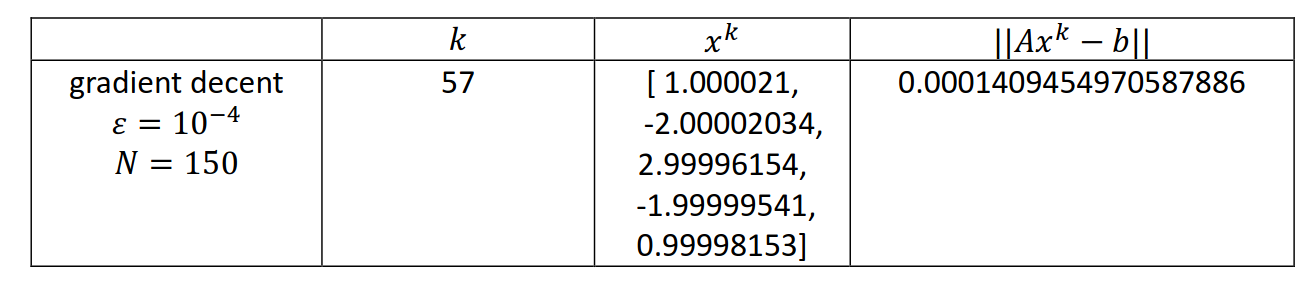
\includegraphics[scale=0.25]{data/ew1}
  \end{figure}
  We minimized the function $f(x) = \half x^T A x - b^T x$ which is equivalent
  to finding a solution to $Ax - b =0$.
  The exact solution is $x = (1,-2,3,-2,1)$.
\item[(2)]
  \begin{figure}[H]
    \centering
    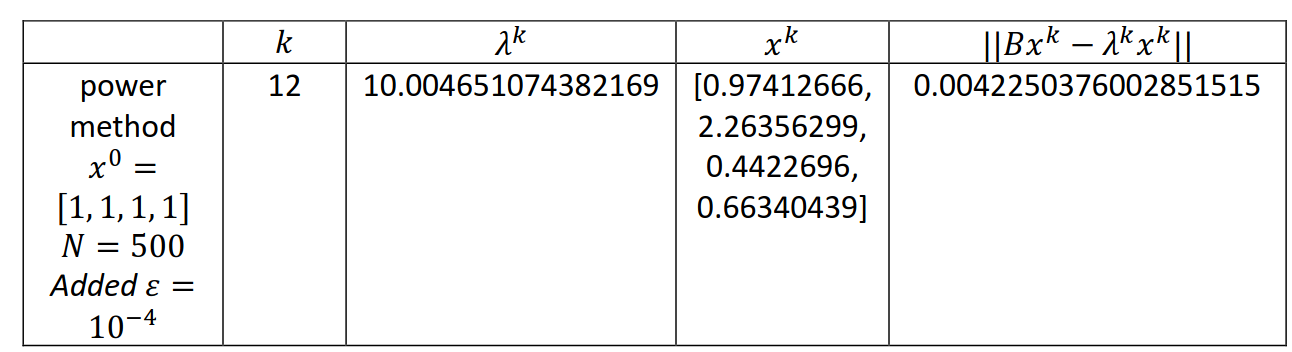
\includegraphics[scale=0.25]{data/ew2}
  \end{figure}
  There's a convergence for $\lambda = 10$ and the eigenvector in
  $\mathrm{span}\set{(194,451,88,132)}$.
\item[(3)]
  \begin{figure}[H]
    \centering
    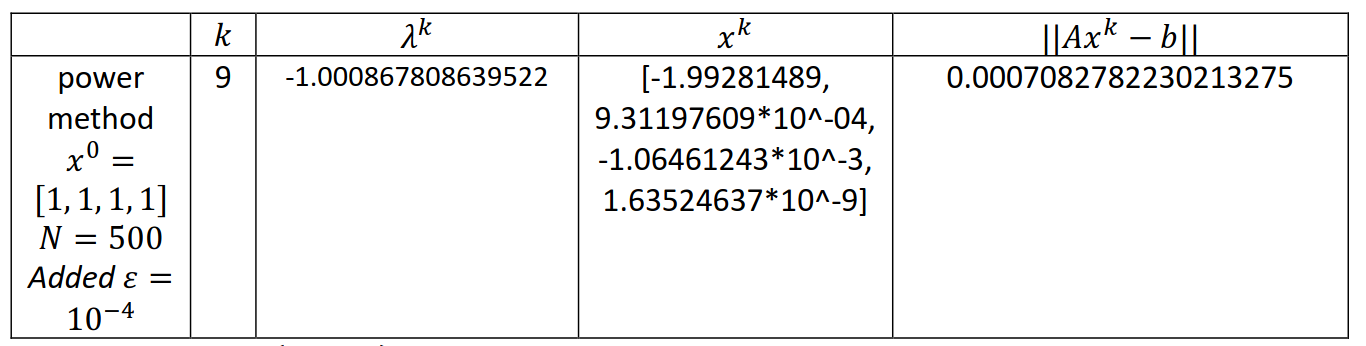
\includegraphics[scale=0.25]{data/ew3}
  \end{figure}
  There's a convergence for $\lambda = -1$ and the eigenvector in
  $\mathrm{span}\set{(1,0,0,0)}$.
\end{solution}


\end{document}
